\lhead{\emph{Partial Sorted Insert Strategy}}
\chapter{Partial Sorted Insert Strategy}
In this section, we will delve into the implementation details of partial sorted insertion strategy and explore various operations such as insertion, update, and deletion. Understanding these fundamental aspects will provide a comprehensive understanding of how partially sorted handles new key insertion.
\section{Implementation Details}

\subsection{The Insertion Algorithm}




\begin{figure}[H]
    \centering
    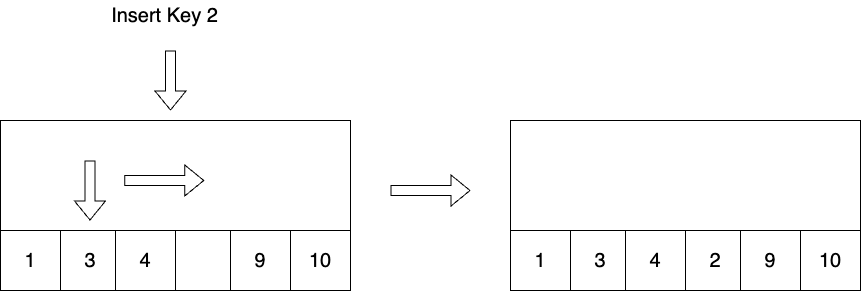
\includegraphics[width=120mm,scale=1]{Figures/PartialSortedInsertion.png}
    \caption{
     Example of Partially Sorted Insertion Strategy
    }
    \label{fig:PartialInsertionExample}
\end{figure}

When it comes to inserting a new key in the partially sorted gapped array of the \acrshort{lipp} index, the process differs from that of a fully sorted array. Instead of creating a new node in the tree for the key, the algorithm must search for the next available gap within the specified limit to insert the new key. This approach is designed to reduce the memory overhead of the \learnindex data structure, as it eliminates the need to create new nodes for every new key.

Specifically, the algorithm traverses down the tree until it reaches a node containing a key that is within the predicted position of the new key. Once such a node is found, the algorithm scans forward within the array for the next available gap to insert the new key. This process ensures that the new key is inserted in the correct position in the partially sorted array, without requiring the creation of new nodes in the tree.
\begin{algorithm}
\caption{Partially Sorted Insertion Strategy}
\begin{algorithmic}[1]

% \State $\texttt{MAX_DEPTH} \gets 128$
\Procedure{insert}{node, key}
\State $current\_node \gets node$
\State $path\_size[]$
\While{$node \neq null$}
\State $pos \gets PREDICT\_POS(current\_node, key)$
\If{$pos$ is child node}
    \State $current node \gets node[pos]$
    \State $path\_size[i] \gets node$
\Else
    \State $key\_pos = PREDICT\_POS(current\_node, key)$
    \If{$node[key\_pos]$ is not empty} 
        \State $key\_pos \gets search\_next\_\epsilon(key\_pos)$
    \EndIf
    $node[key\_pos] \gets key $
    % \State update $frequency\_array$
\EndIf
\EndWhile
\For{$i \gets 0$ to $path\_size - 1$}
   \State $node \gets path[i]$
    \If{rebuilding criteria}
        \State $keys \gets collect\_keys$
        \State $new\_node \gets rebuild\_tree$
        \State $path\_size[i] \gets new\_node$
    \EndIf
\EndFor

\EndProcedure
\end{algorithmic}
\end{algorithm}
However, this approach does have a potential downside in terms of computational overhead. Since the partially sorted array is not fully ordered, the algorithm may need to search further than it would in a fully sorted array to find an available gap to insert the key. This extra search can add additional computational complexity to the insertion process, as the algorithm must spend more time searching for an available gap in the array.

To handle conflicts, partially sorted \learnindex needs to iterate $\epsilon$ spaces after predicted position to collect all the partially sorted keys. This process can be time-consuming, especially if the data set is large. In some cases, the algorithm may need to rebuild the whole node entirely to properly sort the partially sorted keys. As seen from the example Figure \ref{fig:PartialInsertionExample}, if a key $2$ is inserted into an existing tree, it will search for an empty space after the predicted position $1$ and insert the key into the empty location. However, it will only search for $\epsilon$ amount of spaces.

A specific example of this can be seen in the context of a gapped array. When the predicted position contains a partially sorted keys, this requires the algorithm to recursive rebuild of both keys. In such cases, the algorithm needs to iterate through the gapped array to collect all the partially sorted keys that may be located $\epsilon$ distance away from the predicted position.

Moreover, rebuilding the gapped array becomes necessary if the predicted position is itself a partially sorted key. In this scenario, a recursive rebuilding process must be undertaken to ensure that the gapped array is correctly sorted, which will also affect the running time of this algorithm.

As mentioned earlier, one approach to handling conflicts in a gapped array data structure is to use a recursive rebuilding approach. However, an alternative approach is to use the percentage of partially sorted keys to determine whether to rebuild the whole node.

This approach takes advantage of the fact that when a high percentage of the keys in a gapped array is partially sorted, it may be more efficient to rebuild the whole node rather than to attempt to rebuild when the \conflict happens. If the number of partially sorted keys is more than $\frac{1}{2}$ of the number of gapped array lengths, then rebuilding the whole node should be considered.

However, it is essential to note that this approach has limitations and may not always be the most efficient way to handle conflicts in a gapped array. It is also essential to consider other factors, such as the size of the data set and the computational resources available.

In this particular work, we will only be tested on the recursive rebuilding approach. This decision was likely made to simplify the testing process and to provide a clear comparison between baseline and partially sorted gapped array. 


\subsection{The Query Algorithm}

\begin{figure}[H]
    \centering
    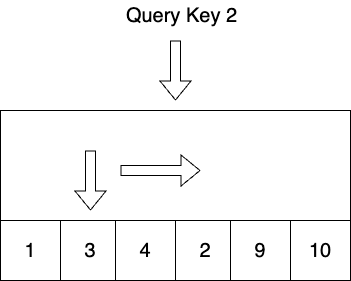
\includegraphics[width=70mm,scale=1]{Figures/QueryPartial.png}
    \caption{
     Example of Partially Sorted Query
    }
    \label{fig:PartialQueryExample}
\end{figure}
When it comes to querying a key in the partially sorted gapped array of the \learnindex algorithm, the process is similar to that of insertion. Like insertion, the algorithm must traverse down the tree until it reaches a node containing a key that is within the predicted position of the queried key. If the key in the node is not the same as the queried key, the algorithm must then scan forward within the array up to the specified limit.

This approach efficiently locates the queried key within the partially sorted array while minimizing the memory overhead of the \learnindex data structure. By accurately predicting the position of the queried key using the linear regression model, the algorithm can quickly navigate the gapped array and locate the keys within the partially sorted limit.
\begin{algorithm}
\caption{Partially Sorted Query}
\begin{algorithmic}[1]
\Procedure{query}{node, key}
\State $current\_node \gets node$
\While{$node \neq null$}
\State $pos \gets PREDICT\_POS(current\_node, key)$
\If{$pos$ is child node}
    \State $current node \gets node[pos]$
    
\Else
    \State $key\_pos = PREDICT\_POS(current\_node, key)$
    \If{$key\_pos \neq key$}
        \State $key\_pos \gets search\_next\_epsilon(current node, key)$
    \EndIf
    \State \Return $node[key\_pos]$
\EndIf
\EndWhile
\State return null
\EndProcedure
\end{algorithmic}
\end{algorithm}
However, scanning forward in the array can potentially add computational complexity to the querying process, mainly if the limit specified is far from the predicted position of the queried key. The algorithm must search through the array to find the next available gap within the limit, which can result in additional computational overhead. 

As an example in Figure \ref{fig:PartialQueryExample}, if searching for $2$, which is a partially sorted key, the predicted position by the model will be the same as insertion, which is $pos \gets 1$. However, the algorithm must perform a sequential search for $\epsilon$ spaces after the predicted position to get key $2$.


\subsection{The Deletion Algorithm}

\begin{figure}[H]
    \centering
    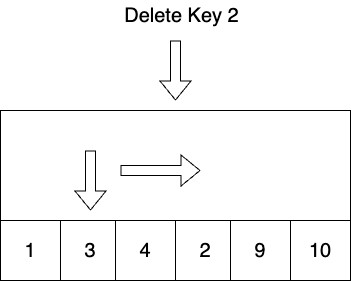
\includegraphics[width=70mm,scale=1]{Figures/PartialSortedDelete.png}
    \caption{
     Example of Partially Sorted Delete
    }
    \label{fig:PartialSortedDeleteExample}
\end{figure}
When it comes to deletion in a data structure such as a \learnindex, the process typically involves searching for specific keys that need removal. However, in the case of a partially sorted gapped array structure, this search process can be more complex, as the keys are not necessarily contiguous and may be spread out over multiple sections of the array.

To perform deletion efficiently in a partially sorted gapped array, the \learnindex algorithm must continue searching for the target keys beyond the predicted location. This typically involves searching until the $\epsilon$ partial sorted limit, where $\epsilon$ is the number of empty spaces after the predicted position the keys can be inserted into.
\begin{algorithm}
\caption{Partially Sorted Delete}
\begin{algorithmic}[1]
\Procedure{delete}{node, key}
\State $current\_node \gets node$
\While{$node \neq null$}
\State $pos \gets PREDICT\_POS(current\_node, key)$
\If{$pos$ is child node}
    \State $current node \gets node[pos]$
    
\Else
    \State $key\_pos = PREDICT\_POS(current\_node, key)$
    \If{$key\_pos \neq key$}
        \State $key\_pos \gets search\_next\_epsilon(current node, key)$
    \EndIf
    \State delete $node[key\_pos]$
\EndIf
\EndWhile
\EndProcedure
\end{algorithmic}
\end{algorithm}

By continuing the search process this way, the \learnindex can ensure that it locates all of the relevant keys for deletion, regardless of their position within the array. This can be a highly efficient method for performing deletions in large datasets, as it avoids the need for costly full scans of the entire array and instead focuses on the relevant sections of the data structure.

As an example, in Figure \ref{fig:PartialSortedDeleteExample}, deleting the keys works similar to query as it has to perform sequential search to find the key that has to be deleted. In this case, the predicted position of key $2$ is $1$ but the algorithm has to search for $\epsilon$ spaces after the predicted position to get the location of key $2$.
\subsection{The Range Query Algorithm}
\begin{algorithm}

\caption{Partially Sorted Query}
\begin{algorithmic}[1]

\Procedure{range\_query}{root, lower, upper}
  \State $stack \gets \text{empty stack}$
  \State $current\_node \gets root$
  \State $keys \gets \text{empty array}$
  \While{$current\_node \neq \text{null}$ \textbf{ or } $stack$ is not empty}
    \While{$current\_node \neq \text{null}$}
      \State $\text{push } current\_node \text{ to } stack$
      \State $pos \gets \text{PREDICT\_POS}(current\_node, \text{lower})$
      \If{$pos$ is a child node}
        \State $current\_node \gets current\_node[pos]$
      \Else
        \State \textbf{break}
      \EndIf
    \EndWhile
    \If{$\text{stack}$ is not empty}
      \State $current\_node \gets \text{pop a node from } stack$
      \State $key\_pos \gets \text{PREDICT\_POS}(current\_node, \text{lower})$
      \For{$i \gets \text{key\_pos}$ to $\text{node\_size}-1$}
        \If{$\text{node}[i] \leq \text{upper}$}
          \State $\text{append } \text{node}[i] \text{ to } keys$
        \Else
          \State \textbf{break}
        \EndIf
      \EndFor
      \State $current\_node \gets current\_node[\text{next position}]$
    \EndIf
  \EndWhile
  \State $collect\_keys\_\epsilon(current node, keys)$
  \State \textbf{return} $keys$
\EndProcedure
\end{algorithmic}
\end{algorithm}
Typically, when performing a range query on a partially sorted gapped array, the algorithm will search for the first key within the specified range and then iterate through the array, collecting all keys until it reaches the end key. However, even after reaching the end key, there may still be additional keys that fall within the specified range but are located in the $\epsilon$ spaces beyond the end key.

The algorithm must continue searching beyond the end key, ensuring that all relevant keys are included in the range query, considering these additional $\epsilon$ spaces. By doing so, the algorithm can identify any keys not included in the initial search but are still within the specified range, providing a comprehensive and accurate result set.


\subsection{The Adjustments Algorithm}
When it comes to working with partially sorted items, several challenges can arise. One of the most significant is that the items are not sorted, and the keys may not follow a consistent, monotonically increasing pattern. This can make it difficult for models to accurately predict the partially sorted keys, leading to inaccuracies in any adjustments made to the item.

To address this issue, one practical approach is to collect all of the keys that need to be rebuilt and retrain the model based on the data collected. By carefully analyzing the information gathered, we can identify patterns and trends that can help us create a more accurate and reliable model. This can involve everything from reviewing historical data to conducting extensive data analysis and modelling exercises.

Another strategy that can be used in the adjustments process is to mix the histogram strategy. This statistical method is used to estimate the distribution of a set of data, which can help us to place gaps between different keys in the item more accurately. By doing so, we can ensure that our adjustments are more precise and that the item is better suited to meet the needs of its intended use.

To simplify the process, we have decided to use \acrfull{ols} as the sole training method for rebuilding the partially sorted \learnindex.

\section{Theoretical Analysis}\label{partialsortedtheory}
\begin{table}
    \centering
    \begin{tabular}{ |p{4cm}|p{3cm}|p{3cm}|  } 
        
     \hline
     \multicolumn{3}{|c|}{Time Complexity} \\
     \hline
      & Partially Sorted & Histogram \\
     \hline
      Insertion Operation & $O(\epsilon + \log N)$ & $O(\log^2 N)$ \\
     \hline
      Query Operation &  $O(\epsilon + \log N)$ & $O(\log N)$ \\
      \hline
      Delete Operation &  $O(\epsilon + \log N)$ & $O(\log N)$ \\
      \hline
      Adjustment Operation & $O(N\log N + \epsilon)$ &  $O(N\log N)$ \\
      \hline
    \end{tabular}
     \caption{Time Complexity of Partially Sorted and Histogram\learnindex}
    \label{tab:timecomplexitypartiallysorted}
\end{table}

Insertion operations for a partially sorted array require the algorithm to search for an empty space before inserting the new key. This search operation takes $O(\log N)$ time, where $N$ is the number of keys in the \learnindex. The new key can be inserted immediately if an empty space is found.

However, if the space is not empty, the algorithm must perform a search for $\epsilon$ spaces after the predicted position to find a suitable location for the new key. This operation takes $O(\epsilon + \log N)$ time, where $\epsilon$ is the limited number of spaces after the predicted position.

In the case of rebuilding recursively, the algorithm needs to rebuild nodes with partially sorted keys. This operation takes $O(\frac{N}{2})$ time, where $N$ is the number of keys in the rebuilding nodes. The algorithm needs to split the nodes into two groups and recursively rebuild them until all nodes are fully sorted.

The time complexity of a query operation in a partially sorted array with a \learnindex is dependent on the position of the key in the array. If the key is located in an empty space, the query operation takes $O(\log N)$ time. This is because the algorithm needs to traverse the \learnindex down to the appropriate leaf node and then search for the key within that node.

However, if the predicted position for the key already contains a key, the algorithm needs to perform additional searches to find the appropriate location for the new key. This takes an additional $\epsilon$ amount of time, resulting in a total time complexity of $O(\epsilon + \log N)$. The value of $\epsilon$ depends on the limit we set for the number of spaces the algorithm can search after the predicted position. 

The time complexity of deletion in a partially sorted array with a \learnindex is also $O(\epsilon + \log N)$, where $\epsilon$ is the limited number of spaces after the predicted position that the algorithm searches for the key to be deleted.

The algorithm first traverses the \learnindex to find the appropriate leaf node and then searches for the key to be deleted. If the key is not found at the predicted position, the algorithm will continue searching for $\epsilon$ spaces after the predicted position to find the key. Once the key is found, the algorithm removes it from the partially sorted array.

Since deletion operations do not involve rebuilding the \learnindex, the time complexity remains the same regardless of the distribution of the keys in the \learnindex.

Adjustment operations in a partially sorted learn index involve collecting a specified number of keys and performing \acrshort{ols} to train the model. The time complexity for adjustment operations is $O(N\log N + \epsilon)$, where $N$ is the number of keys collected for the adjustment process.

The most time-consuming part of the adjustment process is training the model using \acrshort{ols}. However, once the model is trained, it does not require retraining until insertion triggers the recursive rebuilding or once the condition of the adjustment is met. 
